\documentclass[submit]{harvardml}

% Put in your full name and email address.
\name{Christopher Hase}
\email{christopher\_hase@g.harvard.edu}

% List any people you worked with.
\collaborators{%
  None
}

% You don't need to change these.
\course{CS281-F17}
\assignment{Assignment \#2 v 1.1}
\duedate{5:00pm October 9, 2017}

\usepackage{url, enumitem}
\usepackage{amsfonts}
\usepackage{listings}
\usepackage{bm}
\usepackage{bbm}

\usepackage{hyperref}
\usepackage{tikz}
\usetikzlibrary{bayesnet}
% Some useful macros.
\newcommand{\given}{\,|\,}
\newcommand{\R}{\mathbb{R}}
\newcommand{\E}{\mathbb{E}}
\newcommand{\var}{\text{var}}
\newcommand{\cov}{\text{cov}}
\newcommand{\N}{\mathcal{N}}
\newcommand{\ep}{\varepsilon}

\newcommand{\Dir}{\text{Dirichlet}}
\newcommand{\Bet}{\text{Beta}}
\newcommand{\Ber}{\text{Bernoulli}}
% Useful macros.
\newcommand{\trans}{\mathsf{T}}
\newcommand{\bx}{\mathbf{x}}
\newcommand{\by}{\mathbf{y}}
\newcommand{\bw}{\mathbf{w}}
\newcommand{\distNorm}{\mathcal{N}}
\newcommand{\bzero}{\mathbf{0}}
\newcommand{\ident}{\mathbb{I}}
\renewcommand{\v}[1]{\mathbf{#1}}

\begin{document}


\noindent \textbf{NOTE:} you must show derivations for your answers unless a question explicitly mentions that no justification is required.

%%%%%%%%%%%%%%%%%%%%%%%%%%%%%%%%%%%%%%%%%%%%%%%%%%%%%%%%
%%%%%%%%%%%%%%%%% PROBLEM 1 %%%%%%%%%%%%%%%%%%%%%%%%%%%%
%%%%%%%%%%%%%%%%%%%%%%%%%%%%%%%%%%%%%%%%%%%%%%%%%%%%%%%%
\input{problems_Gaussian.tex}

\textbf{(a)} $\mathbf{x}=\big[X_1,...,X_D\big]^T$. Using properties of the multivariate normal, we know that $X_i\stackrel{i.i.d.}{\sim}\N(0,1)$. Then, note that $\sqrt{\mathbf{x}^T\mathbf{x}}=\sqrt{\displaystyle\sum_{i=1}^{D}X_i^2}$. First we'll find the distribution of $Y_i=X_i^2$ with support $[0, \infty)$.\\\\\\
$P(Y_i<y_i)=P(X_i^2<y_i)=P(-\sqrt{y_i}<X_i<\sqrt{y_i})$\\\\
$=2P(X_i<\sqrt{y_i})-1=2\Phi(\sqrt{y_i})-1$ (by symmetry of the normal distribution; $\Phi$ is the standard normal CDF)\\\\
$\dfrac{d\big(2\Phi(\sqrt{y_i})-1\big)}{dy_i}=\phi(\sqrt{y_i})\dfrac{1}{\sqrt{y_i}}$ ($\phi$ is the standard normal PDF)\\\\\\
$=\dfrac{1}{\sqrt{2\pi}}y_i^{-\frac{1}{2}}\exp\bigg(-\dfrac{y_i}{2}\bigg)$\\\\\\
This is the PDF for a $\chi^2$ random variable with $1$ degree of freedom, so $Y_i\sim \chi^2_1\Rightarrow X_i^2\sim \chi^2_1$. Now we need to find the distribution of $Z=\displaystyle\sum_{i=1}^{D}X_i^2$ with support $[0,\infty)$. We can do this using the MGF of $Z$.\\\\
MGF$_Z(t)=\displaystyle\prod_{i=1}^{D}$MGF$_{X_i^2}(t)$\\\\\\
$=\displaystyle\prod_{i=1}^{D}(1-2t)^{-\frac{1}{2}}$\\\\\\
$=(1-2t)^{-\frac{D}{2}}$\\\\
This the the MGF of a $\chi^2$ random variable with $D$ degrees of freedom, so $Z\sim\chi^2_D\Rightarrow\displaystyle\sum_{i=1}^{D}X_i^2\sim\chi^2_D$. Lastly, we need to find the distribution of $W=\sqrt{Z}=\sqrt{\displaystyle\sum_{i=1}^{D}X_i^2}$ with support $[0,\infty)$.\\\\
$P(W<w)=P\big(\sqrt{Z}<w\big)$\\\\
$=P\big(Z<w^2\big)$\\\\
$\dfrac{d\Big(P\big(Z<w^2\big)\Big)}{dw}=2wf_Z(w^2)$\\\\\\
$=\dfrac{2^{1-\frac{D}{2}}w^{D-1}}{\Gamma\big(\frac{D}{2}\big)}\exp\bigg(-\dfrac{w^2}{2}\bigg)$\\\\\\
This is the PDF for a $\chi$ random variable with $D$ degrees of freedom, so $W\sim\chi_D$\\\\
$\Rightarrow\sqrt{\displaystyle\sum_{i=1}^{D}X_i^2}=\sqrt{\mathbf{x}^T\mathbf{x}}\sim\chi_D$ and $f_{\sqrt{\mathbf{x}^T\mathbf{x}}}(x)=\dfrac{2^{1-\frac{D}{2}}x^{D-1}}{\Gamma\big(\frac{D}{2}\big)}\exp\bigg(-\dfrac{x^2}{2}\bigg)$

\newpage
%%%%%%%%%%%%%%%%%%%%%%%%%%%%%%%%%%%%%%%%%%%%%%%%%%%%%%%%
%%%%%%%%%%%%%%%%% PROBLEM 2 %%%%%%%%%%%%%%%%%%%%%%%%%%%%
%%%%%%%%%%%%%%%%%%%%%%%%%%%%%%%%%%%%%%%%%%%%%%%%%%%%%%%%
\input{problems_EXP.tex}
\newpage

\textbf{(a)} $\mathbf{X}\in\R^{N\times m}$ with $\mathbf{x}_i\in\R^m$ as the $i$th row of $\mathbf{X}$ and $x_{ij}\in\R$ as the $j$th element of $\mathbf{x}_i$.\\\\
$\mathbf{Y}\in\R^N$ with $Y_i$ as the $i$th element in $\mathbf{Y}$. Then $\mathbf{y}$ is an instance of $\mathbf{Y}$ and $y_i$ is an instance of $Y_i$.\\\\
$\mathbf{w}_1\in\R^m$ with $w_{1j}$ as the $j$th element in $\mathbf{w}_1$.\\\\
$\mathbf{w}_2\in\R^m$ with $w_{2j}$ as the $j$th element in $\mathbf{w}_2$.\\\\
$\pi_i=\sigma(\mathbf{x}_i^T\mathbf{w}_1)$ $\forall$ $i\in\{1,...,N\}$.\\\\
$\lambda_i=\exp(\mathbf{x}_i^T\mathbf{w}_2)$ $\forall$ $i\in\{1,...,N\}$.\\\\
$\bm{\pi}\in\R^N$ is a vector with $\pi_i$ as the $i$th element and $\bm{\lambda}\in\R^N$ is a vector with $\lambda_i$ as the $i$th element.\\\\
$f$ is an unspecified PDF.\\\\
$\mathbbm{1}$ is an indicator function that takes the value $1$ when its input is true.\\\\\\
$P(\mathbf{Y}=\mathbf{y};\bm{\pi},\bm{\lambda})=\displaystyle\prod_{i=1}^{N}(1-\pi_i)^{\mathbbm{1}[y_i=0]}\Bigg(\pi_i\dfrac{f(y_i;\lambda_i)}{1-f(0;\lambda_i)}\Bigg)^{1-\mathbbm{1}[y_i=0]}$\\\\\\
$\Rightarrow\log\big(P(\mathbf{Y}=\mathbf{y};\bm{\pi},\bm{\lambda})\big)=\displaystyle\sum_{i=1}^{N}\mathbbm{1}[y_i=0]\log(1-\pi_i)+\big(1-\mathbbm{1}[y_i=0]\big)\log\Bigg(\dfrac{f(y_i;\lambda_i)}{1-f(0;\lambda_i)}\Bigg)+\big(1-\mathbbm{1}[y_i=0]\big)\log(\pi_i)$\\\\\\
$=\displaystyle\sum_{i=1}^{N}\log(\pi_i)+\mathbbm{1}[y_i=0]\log\Bigg(\dfrac{1-\pi_i}{\pi_i}\Bigg)+\big(1-\mathbbm{1}[y_i=0]\big)\log\Bigg(\dfrac{f(y_i;\lambda_i)}{1-f(0;\lambda_i)}\Bigg)$\\\\\\
$=\displaystyle\sum_{i=1}^{N}\log(\sigma(\mathbf{x}_i^T\mathbf{w}_1))+\mathbbm{1}[y_i=0]\log\Bigg(\dfrac{1-\sigma(\mathbf{x}_i^T\mathbf{w}_1)}{\sigma(\mathbf{x}_i^T\mathbf{w}_1)}\Bigg)+\big(1-\mathbbm{1}[y_i=0]\big)\log\Bigg(\dfrac{f(y_i;\lambda_i)}{1-f(0;\lambda_i)}\Bigg)$\\\\\\
$=\displaystyle\sum_{i=1}^{N}-\log\big(1+\exp(\mathbf{x}_i^T\mathbf{w}_1)\big)+\big(1-\mathbbm{1}[y_i=0]\big)\mathbf{x}_i^T\mathbf{w}_1+\big(1-\mathbbm{1}[y_i=0]\big)\log\Bigg(\dfrac{f(y_i;\lambda_i)}{1-f(0;\lambda_i)}\Bigg)$\\\\\\
$\dfrac{\partial\log\big(P(\mathbf{Y}=\mathbf{y};\bm{\pi},\bm{\lambda})\big)}{\partial w_{1j}}=\displaystyle\sum_{i=1}^{n}-\dfrac{x_{ij}\exp(\mathbf{x}_i^T\mathbf{w}_1)}{1+\exp(\mathbf{x}_i^T\mathbf{w}_1)}+\big(1-\mathbbm{1}[y_i=0]\big)x_{ij}$ $\forall$ $j\in\{1,...,m\}$\\\\\\
$\Rightarrow\dfrac{\partial\log\big(P(\mathbf{Y}=\mathbf{y};\bm{\pi},\bm{\lambda})\big)}{\partial\mathbf{w}_1}=\Bigg[\dfrac{\partial\log\big(P(\mathbf{Y}=\mathbf{y};\bm{\pi},\bm{\lambda})\big)}{\partial w_{11}},...,\dfrac{\partial\log\big(P(\mathbf{Y}=\mathbf{y};\bm{\pi},\bm{\lambda})\big)}{\partial w_{1m}}\Bigg]^T$\\\\\\
We want to find $\mathbf{\hat w}_1^{MLE}$. This will be the $\mathbf{w}_1$ that makes the gradient of the log-likelihood with respect to $\mathbf{w}_1$ equal to $\mathbf{0}$. To find this $\mathbf{w}_1$, we can use a gradient ascent method. For example, we could initialize $\mathbf{w}_1^{(0)}$ and then use:\\\\
$\mathbf{w}_1^{(i+1)}\leftarrow\mathbf{w}_1^{(i)}+\alpha\dfrac{\partial\log\big(P(\mathbf{Y}=\mathbf{y};\bm{\pi},\bm{\lambda})\big)}{\partial\mathbf{w}_1}\big(\mathbf{w}_1^{(i)}\big)$ until convergence ($\alpha\in\R$ is the learning rate).\\\\\\

\textbf{(b)} Let $Y$ be truncated-at-zero Poisson distributed with parameter $\lambda$.\\\\
$P(Y=y;\lambda)=\dfrac{\frac{\exp(-\lambda)\lambda^y}{y!}}{1-\exp(-\lambda)}$\\\\\\
$=\exp\big(-\lambda+y\log(\lambda)-\log(y!)-\log(1-\exp(-\lambda)\big)$\\\\
$=(y!)^{-1}\exp\Big(y\log(\lambda)-\big(\lambda+\log(1-\exp(-\lambda)\big)\Big)$\\\\\\
$\theta=\log(\lambda)$\\\\
$A(\theta)=\exp(\theta)+\log\big(1-\exp(-\exp(\theta)\big)$\\\\
$\phi(y)=y$\\\\
$h(y)=(y!)^{-1}$\\\\
$\theta$ is the natural parameter, $A(\theta)$ is the log-partition function, $\phi(y)$ is the sufficient statistic, and $h(y)$ is the scaling constant. Because we can write the truncated-at-zero Poisson PMF can be written in the form\\ $P(Y=y;\lambda)=h(y)\exp\big(\theta\phi(y)-A(\theta)\big)$, we know that the truncated-at-zero Poisson distribution is a member of the exponential family.\\\\\\

\textbf{(c)} Let $Y\sim$ Pois$(\lambda)$ and $Y_{trunc}$ be truncated-at-zero Poisson distributed with parameter $\lambda$.\\\\
$E(Y_{trunc})=\displaystyle\sum_{y=0}^{\infty}yP(Y_{trunc}=y)$\\\\
$\Rightarrow\big(1-\exp(-\lambda)\big) E(Y_{trunc})=\displaystyle\sum_{y=0}^{\infty}yP(Y=y)=\lambda$\\\\
$\Rightarrow E(Y_{trunc})=\dfrac{\lambda}{1-\exp(-\lambda)}$\\\\\\\\
Var$(Y_{trunc})=E(Y_{trunc}^2)-\big[E(Y_{trunc})\big]^2$\\\\\\
We'll need to solve for $E(Y_{trunc}^2)$.\\\\
$E(Y_{trunc}^2)=\displaystyle\sum_{y=0}^{\infty}y^2P(Y_{trunc}=y)$\\\\
$\Rightarrow\big(1-\exp(-\lambda)\big) E(Y_{trunc}^2)=\displaystyle\sum_{y=0}^{\infty}y^2P(Y=y)=$Var$(Y)+\big[E(Y)\big]^2=\lambda+\lambda^2$\\\\\\
$\Rightarrow E(Y_{trunc}^2)=\dfrac{\lambda+\lambda^2}{1-\exp(-\lambda)}$\\\\\\
Plugging this and the expectation for $Y_{trunc}$ in, we get:\\\\ Var$(Y_{trunc})=\dfrac{\lambda+\lambda^2}{1-\exp(-\lambda)}-\dfrac{\lambda^2}{\big(1-\exp(-\lambda)\big)^2}$\\\\\\\\
Now let $Y_i$ follow a truncated-at-zero Poisson distribution with parameter $\lambda$ $\forall$ $i\in\{1,...,n\}$ and let $\mathbf{Y}\in\R^n$ have $Y_i$ as its $i$th element. Then $\mathbf{y}$ is an instance of $\mathbf{Y}$ and $y_i$ is an instance of $Y_i$.\\\\
$P(\mathbf{Y}=\mathbf{y};\lambda)=\displaystyle\prod_{i=1}^{n}\dfrac{\frac{\exp(-\lambda)\lambda^y_i}{y_i!}}{1-\exp(-\lambda)}$\\\\\\
$\Rightarrow\log\big(P(\mathbf{Y}=\mathbf{y};\lambda)\big)=\displaystyle\sum_{i=1}^{n}-\lambda+y_i\log(\lambda)-\log(y_i!)-\log(1-\exp(-\lambda)\big)$\\\\\\
$=-n\lambda-n\log\big(1-\exp(-\lambda)\big)+n\bar{y}\log(\lambda)-\displaystyle\sum_{i=1}^{n}\log(y_i!)$\\\\\\
$\dfrac{d\log\big(P(\mathbf{Y}=\mathbf{y};\lambda)\big)}{d\lambda}=-n+\dfrac{n}{1-\exp(\lambda)}+\dfrac{n\bar{y}}{\lambda}$\\\\\\
We want to find $\hat\lambda_{MLE}$. This will be the $\lambda$ that makes the derivative of the log-likelihood with respect to $\lambda$ equal to $0$. To find this $\lambda$, we can use a gradient ascent method. For example, we could initialize $\lambda^{(0)}$ and then use:\\\\
$\lambda^{(i+1)}\leftarrow\lambda^{(i)}+\alpha\dfrac{d\log\big(P(\mathbf{Y}=\mathbf{y};\lambda)\big)}{d\lambda}\big(\lambda^{(i)}\big)$ until convergence ($\alpha\in\R$ is the learning rate).\\\\\\\\


\textbf{(d)} $f(y_i;\lambda_i)=\dfrac{\exp(-\lambda_i)\lambda_i^{y_i}}{y_i!}$ with $\lambda_i=\exp(\mathbf{x}_i^T\mathbf{w}_2)$ $\forall$ $i\in\{1,...,n\}$\\\\
The rest of the notation is the same as in part \textbf{(a)}.\\\\\\
$P(Y_i=y_i;\pi_i,\lambda_i)=(1-\pi_i)^{\mathbbm{1}[y_i=0]}\Bigg(\pi_i\dfrac{\frac{\exp(-\lambda_i)\lambda_i^{y_i}}{y_i!}}{1-\exp(-\lambda_i)}\Bigg)^{1-\mathbbm{1}[y_i=0]}$\\\\\\
$=\exp\Big(\mathbbm{1}[y_i=0]\log(1-\pi_i)+\big(1-\mathbbm{1}[y_i=0]\big)\log(\pi_i)\Big)\exp\Big(-\lambda_i\big(1-\mathbbm{1}[y_i=0]\big)+y_i\big(1-\mathbbm{1}[y_i=0]\big)\log(\lambda_i)-\big(1-\mathbbm{1}[y_i=0]\big)\log(y_i!)-\big(1-\mathbbm{1}[y_i=0]\big)\log\big(1-\exp(-\lambda_i)\big)\Big)$\\\\\\\\
$=\exp\Bigg(\mathbbm{1}[y_i=0]\log\bigg(\dfrac{1-\pi_i}{\pi_i}\bigg)+\log(\pi_i)\Bigg)\exp\big(y_i\log(\lambda_i)-\lambda_i-\log(y_i!)\big)\exp\big(\lambda_i\mathbbm{1}[y_i=0]-y_i\mathbbm{1}[y_i=0]\log(\lambda_i)+\mathbbm{1}[y_i=0]\log(y_i!)\big)\exp\bigg(\big(\mathbbm{1}[y_i=0]-1\big)\Big(\log\big(\exp(\lambda_i)-1\big)-\lambda_i\Big)\bigg)$\\\\\\
$=\exp\Bigg(\mathbbm{1}[y_i=0]\log\bigg(\dfrac{1-\pi_i}{\pi_i}\bigg)+\log(\pi_i)\Bigg)\exp\big(y_i\log(\lambda_i)-\lambda_i-\log(y_i!)\big)\exp\big(\lambda_i\mathbbm{1}[y_i=0]-y_i\mathbbm{1}[y_i=0]\log(\lambda_i)+\mathbbm{1}[y_i=0]\log(y_i!)\big)\exp\bigg(\mathbbm{1}[y_i=0]\log\big(\exp(\lambda_i)-1\big)-\lambda_i\mathbbm{1}[y_i=0]-\log\big(\exp(\lambda_i)-1\big)+\lambda_i\bigg)$\\\\\\
The terms $y_i\mathbbm{1}[y_i=0]\log(\lambda_i)$ and $\mathbbm{1}[y_i=0]\log(y_i!)$ will always be equal to $0$, regardless of the value of $y_i$. Continuing, we have:\\\\\\
$=(y_i!)^{-1}\exp\Bigg(\mathbbm{1}[y_i=0]\bigg(\log\bigg(\dfrac{1-\pi_i}{\pi_i}\bigg)+\log\big(\exp(\lambda_i)-1\big)\bigg)+y_i\log(\lambda_i)-\Big(\log\big(\exp(\lambda_i)-1\big)-\log(\pi_i)\Big)\Bigg)$\\\\\\
$=h(y_i)\exp\big(\bm{\theta}^T\bm{\phi}(y_i)-A(\bm{\theta})\big)$\\\\\\
$\bm{\theta}=[\theta_1$, $\theta_2]^T=\Bigg[\log\bigg(\dfrac{1-\pi_i}{\pi_i}\bigg)+\log\big(\exp(\lambda_i)-1\big)$, $\log(\lambda_i)\Bigg]^T$\\\\\\
$=\Bigg[\log\bigg(\dfrac{1-\sigma(\mathbf{x}_i^T\mathbf{w}_1)}{\sigma(\mathbf{x}_i^T\mathbf{w}_1)}\bigg)+\log\Big(\exp\big(\exp(\mathbf{x}_i^T\mathbf{w}_2)\big)-1\Big)$, $\mathbf{x}_i^T\mathbf{w}_2\Bigg]^T$\\\\\\
$=\bigg[\log\Big(\exp\big(\exp(\mathbf{x}_i^T\mathbf{w}_2)\big)-1\Big)-\mathbf{x}_i^T\mathbf{w}_1$, $\mathbf{x}_i^T\mathbf{w}_2\bigg]^T$\\\\\\
$A(\bm{\theta})=\log\Big(\exp(\theta_1)+\exp\big(\exp(\theta_2)\big)-1\Big)$\\\\
$\bm{\phi}(y_i)=[\mathbbm{1}[y_i=0]$, $y_i$]\\\\
$h(y_i)=(y_i!)^{-1}$\\\\
$\bm{\theta}$ represents the the natural parameters, $A(\bm{\theta})$ is the log-partition function, $\bm{\phi}(y_i)$ represents the sufficient statistics, and $h(y_i)$ is the scaling constant. Because we can write the hurdle model PMF for $Y_i$ in the exponential family form $P(Y_i=y_i;\pi_i,\lambda_i)=h(y_i)\exp\big(\bm{\theta}^T\bm{\phi}(y_i)-A(\bm{\theta})\big)$, we know that the hurdle model is a valid GLM.\\\\
Now we need to derive the log-likelihood for the hurdle model GLM. Starting from the final log-likelihood expression in part \textbf{(a)}, we have:\\
$\log\big(P(Y_i=y_i;\pi_i,\lambda_i)\big)=-\log\big(1+\exp(\mathbf{x}_i^T\mathbf{w}_1)\big)+\big(1-\mathbbm{1}[y_i=0]\big)\mathbf{x}_i^T\mathbf{w}_1+\big(1-\mathbbm{1}[y_i=0]\big)\log\Bigg(\dfrac{\frac{\exp(-\lambda_i)\lambda_i^{y_i}}{y_i!}}{1-\exp(-\lambda_i)}\Bigg)$\\\\
$=-\log\big(1+\exp(\mathbf{x}_i^T\mathbf{w}_1)\big)+\big(1-\mathbbm{1}[y_i=0]\big)\mathbf{x}_i^T\mathbf{w}_1+\big(1-\mathbbm{1}[y_i=0]\big)\Big(y_i\log(\lambda_i)-\big(\lambda_i+\log\big(1-\exp(-\lambda_i)\big)\big)-\log(y_i!)\Big)$
$=-\log\big(1+\exp(\mathbf{x}_i^T\mathbf{w}_1)\big)+\big(1-\mathbbm{1}[y_i=0]\big)\mathbf{x}_i^T\mathbf{w}_1+\big(1-\mathbbm{1}[y_i=0]\big)\Big(y_i\mathbf{x}_i^T\mathbf{w}_2-\big(\exp(\mathbf{x}_i^T\mathbf{w}_2)+\log\big(1-\exp(-\exp(\mathbf{x}_i^T\mathbf{w}_2))\big)\big)-\log(y_i!)\Big)$


%%%%%%%%%%%%%%%%%%%%%%%%%%%%%%%%%%%%%%%%%%%%%%%%%%%%%%%%
%%%%%%%%%%%%%%%%% PROBLEM 3  %%%%%%%%%%%%%%%%%%%%%%%%%%%
%%%%%%%%%%%%%%%%%%%%%%%%%%%%%%%%%%%%%%%%%%%%%%%%%%%%%%%%
\input{problems_GM.tex}

\textbf{(a)} $N$ is the number of data points.\\\\
$P(y,x_1,x_2,x_3,x_4)=P(y|x_1,x_2,x_3,x_4)\cdot P(x_1|x_2,x_3,x_4)\cdot P(x_2|x_3,x_4)\cdot P(x_3|x_4)\cdot P(x_4)$
\begin{center}
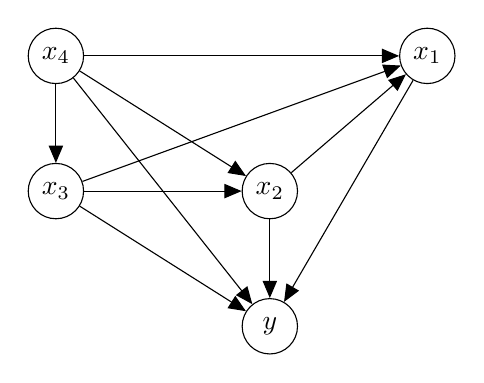
\begin{tikzpicture}
  %Define nodes
  \node[latent] (y) {$y$};
  \node[latent, above= of y]  (x2) {$x_2$};
  \node[latent, left=2cm of x2] (x3) {$x_3$};
  \node[latent, above=of x3] (x4) {$x_4$};
  \node[latent, right=4cm of x4] (x1) {$x_1$};

  % Connect the nodes
  \edge {x1, x2, x3, x4} {y};
  \edge {x2, x3, x4} {x1};
  \edge {x3, x4} {x2};
  \edge {x4} {x3};

\end{tikzpicture}
\end{center}

\textbf{(b)} The size of the conditional probability tables will be $C\cdot2^4$ for $y|x_1,x_2,x_3,x_4$,  $2^4$ for $x_1|x_2,x_3,x_4$,  $2^3$ for $x_2|x_3,x_4$, $2^2$ for $x_3|x_4$. Then the sum of the sizes of the conditional probability tables will be $C\cdot2^4+2^4+2^3+2^2=16C+28$. The size of the marginal probability table for $x_4$ is $2$, so the sum of the sizes of all the probability tables will be $16C+30$.\\\\
Without assuming independence or conditional independence, we cannot reduce the magnitude of this value with a different DGM. Any valid factorization of the joint PDF into univariate distributions where $y|x_1,x_2,x_3,x_4$ is included in the factorization will necessarily yield the same sized conditional probability tables if we do not make independence or conditional independence assumptions.\\\\

\textbf{(c)} $X_1|Y,...,X_V|Y$ are independent. Then the DGM can be represented by the following graph:
\begin{center}
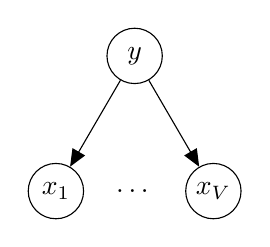
\begin{tikzpicture}
  %Define nodes
  \node[latent] (y) {$y$};
  \node[latent, below=of y, xshift=-1cm]  (x1) {$x_1$};
  \node[latent, below=of y, xshift=1cm]  (xv) {$x_V$};

  % Connect the nodes
  \edge {y} {x1};
  \edge {y} {xv};
  
  \path (x1) -- node[auto=false]{\ldots} (xv);

\end{tikzpicture}
\end{center}
Each conditional probability table will be size $2C$, so the sum of the sizes of the conditional probability tables will be $2CV$. The size of the marginal probability table for $y$ is $C$, so the sum of the sizes of all the probability tables will be $2CV+C$.\\\\

\textbf{(d)} $\theta\sim$ Dir$(\alpha)$ with $\theta,\alpha\in\R^C$. This the prior for the distribution of class labels.\\\\
$Y^{(n)}|\theta\sim$ Cat$(\theta)$ with $Y^{(n)}\in\R^C$ as a one hot encoded vector such that $Y_c^{(n)}=1$ if the $n$th data point has class label $c$ and $0$ otherwise.\\\\
$\beta_{cv}\sim$ Beta$(\beta_{0cv},\beta_{1cv})$ with $\beta_{cv},\beta_{0cv},\beta_{1cv}\in\R$. This is the prior for the $v$th feature for data points that have class label $c$.\\\\
$X_v^{(n)}|\beta_{cv}\sim$ Bern$\big(\beta_{cv}\big)$\\\\\\\\\\\\\\\\
The DGM can then be represented by the following graph:
\begin{center}
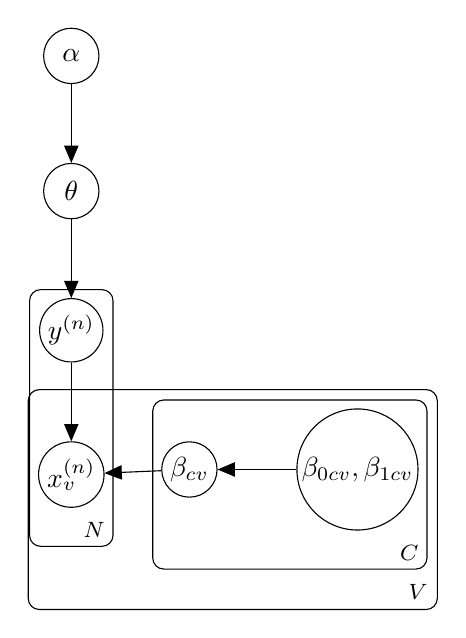
\begin{tikzpicture}
  %Define nodes
  \node[latent] (alpha) {$\alpha$};
  \node[latent, below=of alpha]  (theta) {$\theta$};
  \node[latent, below=of theta]  (y) {$y^{(n)}$};
  \node[latent, below=of y, xshift=1.5cm]  (beta) {$\beta_{cv}$};
  \node[latent, right=1cm of beta]  (betacv) {$\beta_{0cv},\beta_{1cv}$};
  \node[latent, below=of y]  (x) {$x_v^{(n)}$};

  % Connect the nodes
  \edge {alpha} {theta};
  \edge {theta} {y};
  \edge {y} {x};
  \edge {beta} {x};
  \edge {betacv} {beta};
  
  % Plates
  \plate [inner sep =0.1cm] {C} {(betacv)(beta)} {$C$};
  \plate {V} {(x)(C)} {$V$};
  \plate [inner sep = 0.1cm] {N} {(y)(x)} {$N$};
  

\end{tikzpicture}
\end{center}
Note that $\beta_{cv}$ is used to generate $x_v^{(n)}\Leftrightarrow y^{(n)}_c = 1$. Otherwise it is ignored.\\\\

\textbf{(e)}\\\\
\textbf{(1)} False. The path from feature $x_1^{(n)}$ to $x_2^{(n)}$ through $y^{(n)}$ is not blocked.\\\\
\textbf{(2)} False. The path from the class labels to the class-conditional parameters through the features is not blocked when the features are in the evidence.\\\\
\textbf{(3)} True. The path from $y^{(i)}$ to $y^{(j)}$ through $\theta$ is blocked when $\theta$ is in the evidence.\\\\
\textbf{(4)} False. The path from $x_i^{(n)}$ to $x_j^{(n)}$ through $y^{(n)}$ is not blocked when the class distribution parameters are in the evidence.\\\\
\textbf{(5)} False. The path from $y^{(i)}$ to $y^{(j)}$ through $\theta$ is not blocked when $\alpha$ is in the evidence.\\\\\\

\textbf{(f)} A benefit would be that the model captures the fact that there can be multiple instances of each feature in a given example via the class-conditional distributions for each feature. We lose information about a given example by only allowing for binary features. A drawback is that the number of parameters required to fit the model is multiplied by something on the order of $\frac{D}{2}$. As a result, if we don't have a ton of data, we may not be able to achieve a generalizable model fit. A third option would be to model the entire distribution over features for each class using a Dirichlet-Multinomial. This would allow us to capture the fact that there can be multiple instances of each feature in a given example without requiring as many parameters to fit the model.

%%%%%%%%%%%%%%%%%%%%%%%%%%%%%%%%%%%%%%%%%%%%%%%%%%%%%%%%
%%%%%%%%%%%%%%%%% PROBLEM 4 %%%%%%%%%%%%%%%%%%%%%%%%%%%%
%%%%%%%%%%%%%%%%%%%%%%%%%%%%%%%%%%%%%%%%%%%%%%%%%%%%%%%%
\input{problems_NB.tex}
Test accuracy $=0.864$\\
Class prior parameter magnitude = $1$\\
Beta class-conditional prior parameter magnitude = $1$\\\\
Test accuracy $=0.863$\\
Class prior parameter magnitude = $1$\\
Dirichlet class-conditional prior parameter magnitude = $0.4$\\
Note that the maximum number of times that a feature could be drawn to was set to $D=10$ (see \textbf{3(f)})\\\\
The classes are not unbalanced in the dataset, so increasing the relative value of the prior parameter for the less often occurring class is not a relevant question here. If the classes were imbalanced, it still seems that we would want our prior to reflect the truth. That is, if our goal is to maximize accuracy, we would want our posterior mean for the distribution over classes to reflect the distribution over classes for the data we want to make predictions on, and choosing a prior that reflects the distribution over classes for data we want to make predictions on would help to give us such a posterior mean. If we have a goal for our model for which we care about false positives, false negatives, true positives, and true negatives, then we may want to choose a prior with non-uniformity for the distribution over classes to help us achieve that goal.
 
\newpage
%%%%%%%%%%%%%%%%%%%%%%%%%%%%%%%%%%%%%%%%%%%%%%%%%%%%%%%%
%%%%%%%%%%%%%%%%% PROBLEM 5 %%%%%%%%%%%%%%%%%%%%%%%%%%%%
%%%%%%%%%%%%%%%%%%%%%%%%%%%%%%%%%%%%%%%%%%%%%%%%%%%%%%%%
\input{problems_LR.tex}

\textbf{(a)(i)} $\mathbf{X}\in\R^{N\times m}$ with $\mathbf{x}_i\in\R^m$ as the $i$th row of $\mathbf{X}$ and $x_{ij}\in\R$ as the $j$th element of $\mathbf{x}_i$.\\\\
$\mathbf{Y}\in\R^N$ with $Y_i$ as the $i$th element in $\mathbf{Y}$. Then $\mathbf{y}$ is an instance of $\mathbf{Y}$ and $y_i$ is an instance of $Y_i$.\\\\
$\mathbf{W}\in\R^m$ with $W_i$ as the $i$th element in $\mathbf{W}$. Then $\mathbf{w}$ is an instance of $\mathbf{W}$ and $w_i$ is an instance of $W_i$.\\\\
$p(\mathbf{w}|\mathbf{y},\mathbf{X})\propto p(\mathbf{y}|\mathbf{X},\mathbf{w})p(\mathbf{w}|\mathbf{X})$\\\\
$=\displaystyle\prod_{i=1}^{N}p(y_i|\mathbf{x}_i,\mathbf{w})p(\mathbf{w}|\mathbf{x}_i)=p(\mathbf{w})^N\displaystyle\prod_{i=1}^{N}p(y_i|\mathbf{x}_i,\mathbf{w})$\\\\\\
$\Rightarrow\log\big(p(\mathbf{y}|\mathbf{X},\mathbf{w})p(\mathbf{w})\big)=\displaystyle\sum_{i=1}^{N}\log\big(p(y_i|\mathbf{x}_i,\mathbf{w})\big)+N\log\big(p(\mathbf{w})\big)$\\\\\\
$=\displaystyle\sum_{i=1}^{N}\log\big(p(y_i|\mathbf{x}_i,\mathbf{w})\big)-\dfrac{N||\mathbf{w}||_1}{b}-N\log(2b)$\\\\\\
From problem \textbf{2(a)}, we know that this simplifies to:\\\\
$=\displaystyle\sum_{i=1}^{N}-\log\big(1+\exp(\mathbf{x}_i^T\mathbf{w})\big)+y_i\mathbf{x}_i^T\mathbf{w}\mathbf-\dfrac{N||\mathbf{w}||_1}{b}-N\log(2b)$\\\\\\
$\dfrac{\partial\big(p(\mathbf{w}|\mathbf{y},\mathbf{X})\big)}{\partial w_j}=\displaystyle\sum_{i=1}^{n}-\dfrac{x_{ij}\exp(\mathbf{x}_i^T\mathbf{w})}{1+\exp(\mathbf{x}_i^T\mathbf{w})}+y_ix_{ij}-\dfrac{Nw_j}{b|w_j|}$ $\forall$ $j\in\{1,...,m\}$ (case where no $w_i=0$)\\\\\\
$\Rightarrow\dfrac{\partial\big(p(\mathbf{w}|\mathbf{y},\mathbf{X})\big)}{\partial \mathbf{w}}=\Bigg[\dfrac{\partial\big(p(\mathbf{w}|\mathbf{y},\mathbf{X})\big)}{\partial w_1},...,\dfrac{\partial\big(p(\mathbf{w}|\mathbf{y},\mathbf{X})\big)}{\partial w_m}\Bigg]^T$\\\\\\
We want to find $\mathbf{\hat w}^{MAP}$. This will be the $\mathbf{w}$ that makes the gradient of the log-likelihood with respect to $\mathbf{w}$ equal to $\mathbf{0}$. To find this $\mathbf{w}$, we can use a coordinate ascent method.\\\\

\textbf{(a)(ii)} Note that $\mathbf{\hat w}^{MAP}$, which is the $\mathbf{w}$ maximizes $\displaystyle\sum_{i=1}^{N}\log\big(p(y_i|\mathbf{x}_i,\mathbf{w})\big)-\dfrac{N||\mathbf{w}||_1}{b}-N\log(2b)$ (we showed this in part \textbf{(a)(i)}) will be the same $\mathbf{w}$ that minimizes $-\dfrac{1}{N}\displaystyle\sum_{i=1}^{N}\log\big(p(y_i|\mathbf{x}_i,\mathbf{w})\big)+\dfrac{||\mathbf{w}||_1}{b}$ since we modified the first expression by negating it, multiplying by a constant, and deleting a term that did not depend on $\mathbf{w}$. Thus, we can find $\mathbf{\hat w}^{MAP}$ by minimizing the following with respect to $\mathbf{w}$:\\\\
$-\dfrac{1}{N}\displaystyle\sum_{i=1}^{N}\log\big(p(y_i|\mathbf{x}_i,\mathbf{w})\big)+\lambda||\mathbf{w}||_1$ where $\lambda=\dfrac{1}{b}$\\\\\\

\textbf{(b)(i)} Validation accuracy when $\lambda=0:$ $0.858$\\
Validation accuracy when $\lambda=0.001:$ $0.819$\\
Validation accuracy when $\lambda=0.01:$ $0.738$\\
Validation accuracy when $\lambda=0.1:$ $0.557$\\
Validation accuracy when $\lambda=1:$ $0.534$\\
Test accuracy when $\lambda=0:$ $0.860$\\\\

\textbf{(b)(ii)}\\\\
Words with highest valued coefficients for predicting class $0$: ['worst' 'bad' 'waste' 'poor' 'nothing']\\\\
Words with lowest valued coefficients for predicting class $0$: ['great' 'best' 'excellent' 'well' 'loved']\\\\
Words with highest valued coefficients for predicting class $1$: ['great' 'best' 'excellent' 'well' 'loved']\\\\
Words with lowest valued coefficients for predicting class $1$: ['worst' 'bad' 'waste' 'poor' 'nothing']\\\\\\

\textbf{(b)(iii)} Validation accuracy when $\lambda=0:$ $0.858$\\
Validation accuracy when $\lambda=0.001:$ $0.819$\\
Validation accuracy when $\lambda=0.01:$ $0.738$\\
Validation accuracy when $\lambda=0.1:$ $0.557$\\
Validation accuracy when $\lambda=1:$ $0.534$\\\\
Test accuracy when $\lambda=0:$ $0.860$\\
Test accuracy when $\lambda=0.001:$ $0.815$\\
Test accuracy when $\lambda=0.01:$ $0.739$\\
Test accuracy when $\lambda=0.1:$ $0.554$\\
Test accuracy when $\lambda=1:$ $0.522$\\\\\\
Number of $0$ valued parameters for class $0$ ($\lambda=0$): $0.0453$\\
Number of $0$ valued parameters for class $1$ ($\lambda=0$): $0.0462$\\\\
Number of $0$ valued parameters for class $0$ ($\lambda=0.001$): $0.9898$\\
Number of $0$ valued parameters for class $1$ ($\lambda=0.001$): $0.9898$\\\\
Number of $0$ valued parameters for class $0$ ($\lambda=0.01$): $0.995$\\
Number of $0$ valued parameters for class $1$ ($\lambda=0.01$): $0.996$\\\\
Number of $0$ valued parameters for class $0$ ($\lambda=0.1$): $0.0995$\\
Number of $0$ valued parameters for class $1$ ($\lambda=0.1$): $0.0982$\\\\
Number of $0$ valued parameters for class $0$ ($\lambda=1$): $0.0424$\\
Number of $0$ valued parameters for class $1$ ($\lambda=1$): $0.0415$\\\\
When we increase $\lambda$ from $0$ to $0.001$, the sparsity of the parameters increases drastically. It increases still for the increase in $\lambda$ from $0.001$ to $0.01$. However, for the increase in $\lambda$ from $0.01$ to $0.1$ we see a huge drop in sparsity. We then see another drop in sparsity when we increase $\lambda$ from $0.1$ to $1$. The increase in sparsity along with increases in $\lambda$ is what we would expect to see. I suspect that the reason that we see the drops in sparsity for the last two increases in $\lambda$ is that stochastic gradient descent never achieves any sort of convergence to a minimum.


\newpage
%%%%%%%%%%%%%%%%%%%%%%%%%%%%%%%%%%%%%%%%%%%%%%%%%%%%%%%%
%%%%%%%%%%%%%%%%% PROBLEM 6 %%%%%%%%%%%%%%%%%%%%%%%%%%%%
%%%%%%%%%%%%%%%%%%%%%%%%%%%%%%%%%%%%%%%%%%%%%%%%%%%%%%%%
\input{problems_NN.tex}

\textbf{(a)} I implemented a neural network for IMDB classification with one hidden layer of size $\frac{V}{1000}$ ($V$ is the size of the vocabulary) that used a Tanh activation function. I used an SGD optimizer with a learning rate of $0.01$. I used negative log likelihood loss as my loss function.\\\\
Test accuracy = $0.862$

\end{document}
